\documentclass{article}
\usepackage[utf8]{inputenc}
\usepackage[margin=0.70in]{geometry}
\usepackage{hyperref}
\usepackage{graphicx}

\title{CS 267: Enabling GPU Support on NumS}
\author{Brian Park, Kunal Agarwal, Parth Baokar}
\date{May 2022}

\begin{document}

\maketitle

\section*{Abstract}
NumS is a library that translates Python and NumPy to optimized distributed systems code. Originally, it was built on top of Ray and was intended for cloud computing environment. We explore how to implement a GPU backend that can be deployable on HPC systems with multi GPU configurations, such as NVIDIA V100 cluster connected with NVLink. We implement a GPU backend that uses CuPy to execute kernels on NVIDIA GPUs and evaluate the performance on multi GPU setup with Ray and NCCL.

\section{Introduction}
Nowadays, there are many parallel primitives that can be used to accelerate numerical workloads. The most popular ones by far for the CPU have been OpenMP, MPI, and UPC++. But often, CPUs do not meet the demand of compute power coming from deep learning models, often requiring petabytes/s of throughput \cite{openai}. Figure 1 shows that the increase in compute power over the past decade. This is where domain specific hardware is needed, such as GPUs and TPUs to bridge the gap between compute power today's hardware provides and the growing demand from deep learning. But even then, GPUs and TPUs are often limited by high bandwidth memory to store parameters for machine learning. Due to the death of Moore's Law and end of Denard's scaling, distributed systems is often the solution to scale indefinitely. Here, we will analyze and evaluate the performance and design of NumS with single GPU and multi GPU inter-node backends to reach teraflops/s of performance.

\begin{figure}
  \centerline{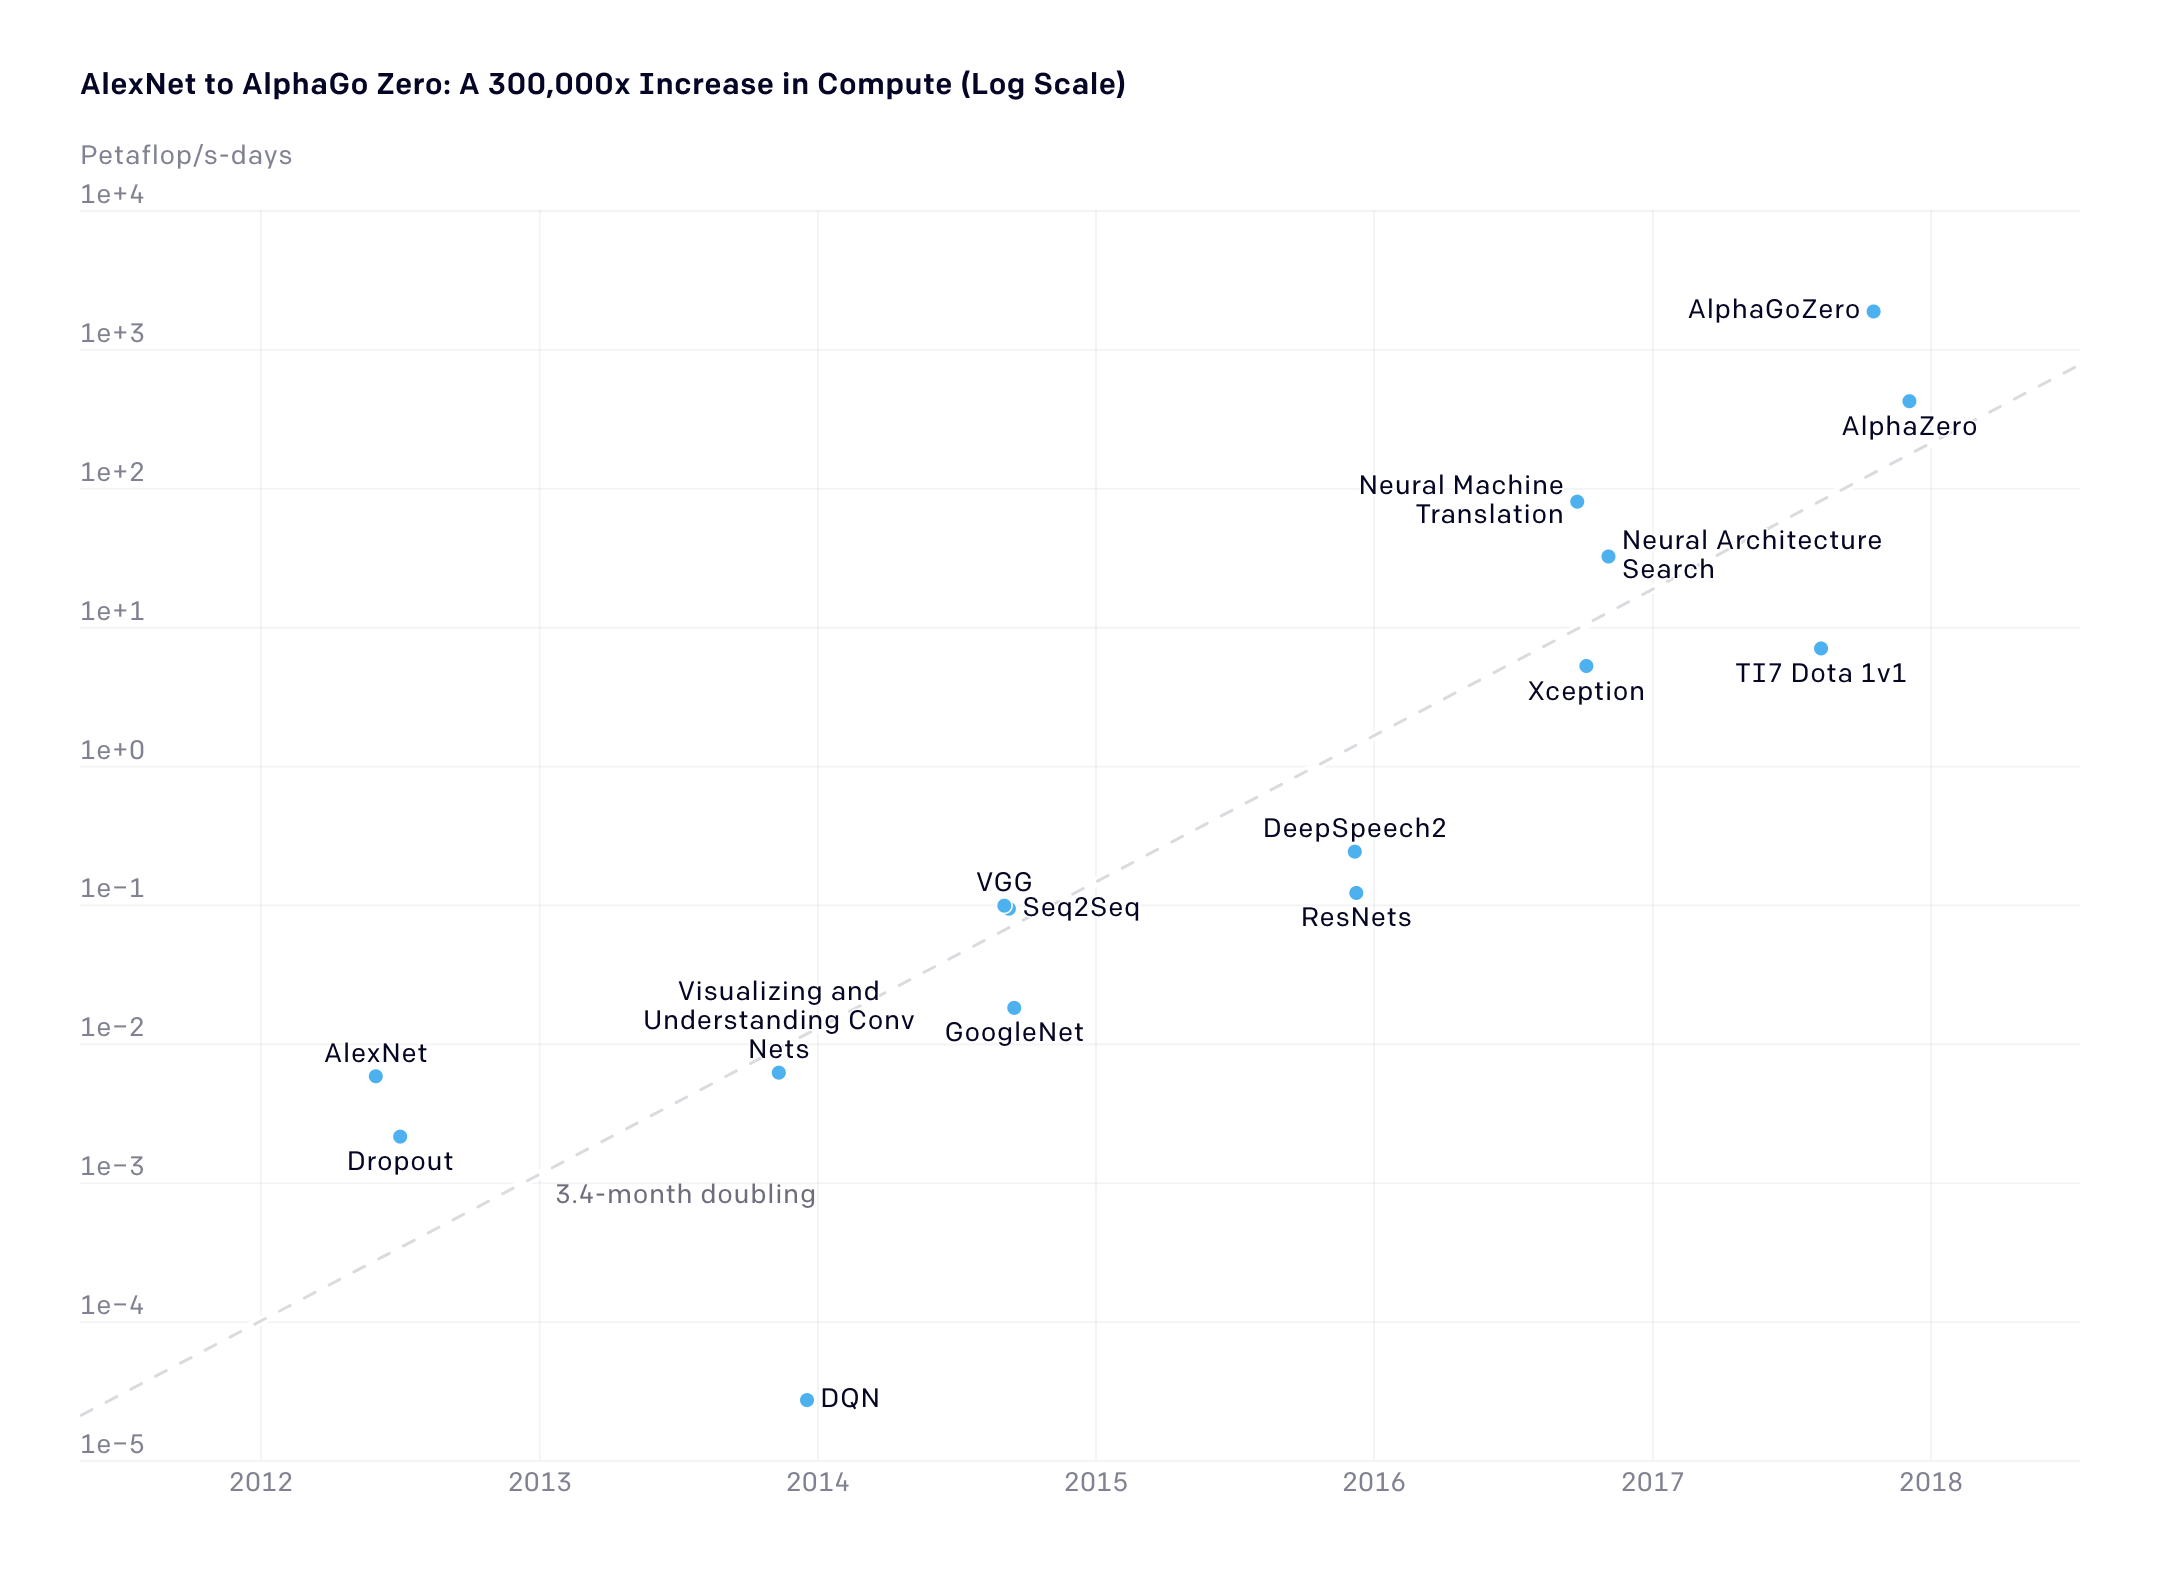
\includegraphics[width=6in]{figures/ai-and-compute-modern-log.png}}
  \caption{Compute Demands of Machine and Deep Learning Models}
\end{figure}

\section{Design}
NumS by design already tries to optimize for distributed systems by providing optimal schedulers and communication avoiding algorithms. \cite{nums} We find that these same algorithms can be easily transferable when implementing a multi GPU backend.

The core backend of NumS uses NumPy for numerical computations and it has a kernel interface where computations are executed by partitions in a map-reduce style of programming. NumS has kernels written in NumPy that execute on each data partition in a SPMD style interface. For communication, an application level interface is used to coordinate data movement between devices. Because it was originally written in Ray, the communication APIs are abstracted away from the developer using Ray's object store. The object store is an in-memory distributed object store, using futures and promises to enable task parallelism \cite{ray}. It abstracts away the communication to the developer, making writing distributed programming simple. NumS is able to be aware of array partitioning, placement, and scheduling by utilizing advanced Ray API functionality.

CuPy is a NumPy/SciPy-compatible array library for GPU-accelerated computing with Python. It can be often used as drop-in replacement for NumPy, and we use it to enable GPU support on NumS. \cite{cupy} Just like how NumPy can use optimized vendor libraries for BLAS like Intel MKL, CuPy uses NVIDIA's cuBLAS on NVIDIA GPUs while also being aware of NVIDIA hardware features such as NVIDIA Tensor Cores. Thus, CuPy serves as a viable option for NumS compared to other array libraries like Dask, Jax, or Numba. This also means that the scope of GPU support on NumS is only limited to NVIDIA GPUs with CUDA support.

Another reason why CuPy serves as a viable option is because it also provides low level CUDA API support such as Python wrappers over the NCCL library. This allows us to write distributed code for NVIDIA GPUs using NCCL as opposed to other options such as CUDA-aware MPI. Another benefit of using NCCL is that it can be used in a single process, where it wont be a problem with Python's global interpreter lock.

Here, we'll explore how we implement GPU support with one GPU and extend it to two more approaches when implementing multi-GPU support with Ray and NCCL. We chose to explore Ray in order to be faithful with the already existing CPU Ray implementation of NumS.

\subsection{Serial}
We implemented the simple serial model, where NumS only uses 1 GPU. This implementation was very simple to implement as we used CuPy as our kernel interface. Properly implementing this gave us a starting point before we extended it to a multi GPU setup. Some basic synchronization primitives have to be implemented such as synchronizing GPU threads and only transferring from GPU memory to main memory when results are needed to be served to the user.

\subsection{Ray}
For implementing the multi-GPU support, we find that Ray's features to abstract away distributed code to the developer and user can be a drawback. Ray's Object Store was meant to be a way to provide a fault tolerant distributed memory model. \cite{ray} This causes a huge latency when doing computations on the GPUs, as Ray enabled functions with CuPy would forcefully route data transfers from CPU to GPU and back from GPU to CPU. This is because Ray exclusively models the Object Store as main memory, and does not include GPU memory in the model. Because low level control is abstracted away, such as explicitly transferring data between nodes or scheduling operations, implementing a high performance GPU backend becomes more of a challenge to implement. Ray was also meant to accelerate task parallelism. Although NumS is successfully able to use Ray features to enable data parallelism computations, Ray's features for data parallelism with GPU is not well supported yet. Ray also provides a collective communication library that can use NCCL to bypass data transfers to the object store. It seems to be successful in Alpa, where they use stateful Ray actor implementations \cite{alpa}. But the design of NumS was built on top of Ray remote functions which are stateless. Trying to incorporate an actor implementation would require a redesign of the NumS system architecture. 

\subsection{NCCL}
With NCCL communication, there are some disadvantages over Ray that NCCL does not supply, such as not being fault tolerant and being susceptible to a deadlock. If a device goes offline in the middle of communication call, this is where NCCL fails to continue, while a Ray implementation can continue on. But since the focus of this implementation was to make NumS deployable under a HPC environment, NCCL served as a better choice in this use case, as these problems are more susceptible in cloud computing. 

When using NCCL, we also had to use multiple CUDA streams to enable concurrency. Naively running code on multiple GPUs will all sync up to the null thread and serialize the timeline and not enable concurrency. For communication under NCCL, we used simple send and receive calls. For future work, we could try to improve the collective communication calls for certain algorithms to utilize other collective calls such as \verb|BCast| and \verb|AllReduce|

\begin{figure}
  \centerline{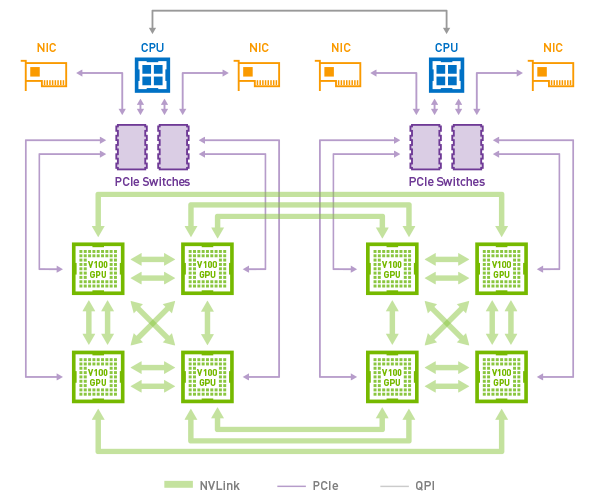
\includegraphics[width=6in]{figures/nvlink.png}}
  \caption{NVLink Mappings in DGX-2 System}
\end{figure}

\section{Evaluation}
This is one of the first applications where NumS has successfully run on a HPC machine environment. Ray was not intended to run on HPC systems, as mentioned in a guest lecture by Ion Stoica. \cite{ray-lecture}. But we see it as a viable option in DGX-2 systems as we are able to achieve scalability with the utilization of NVLink connections. 

\subsection{Profiling}
When naively using just the null CUDA stream, we see that concurency won't be enabled as shown in figure 3

\begin{figure}
  \centerline{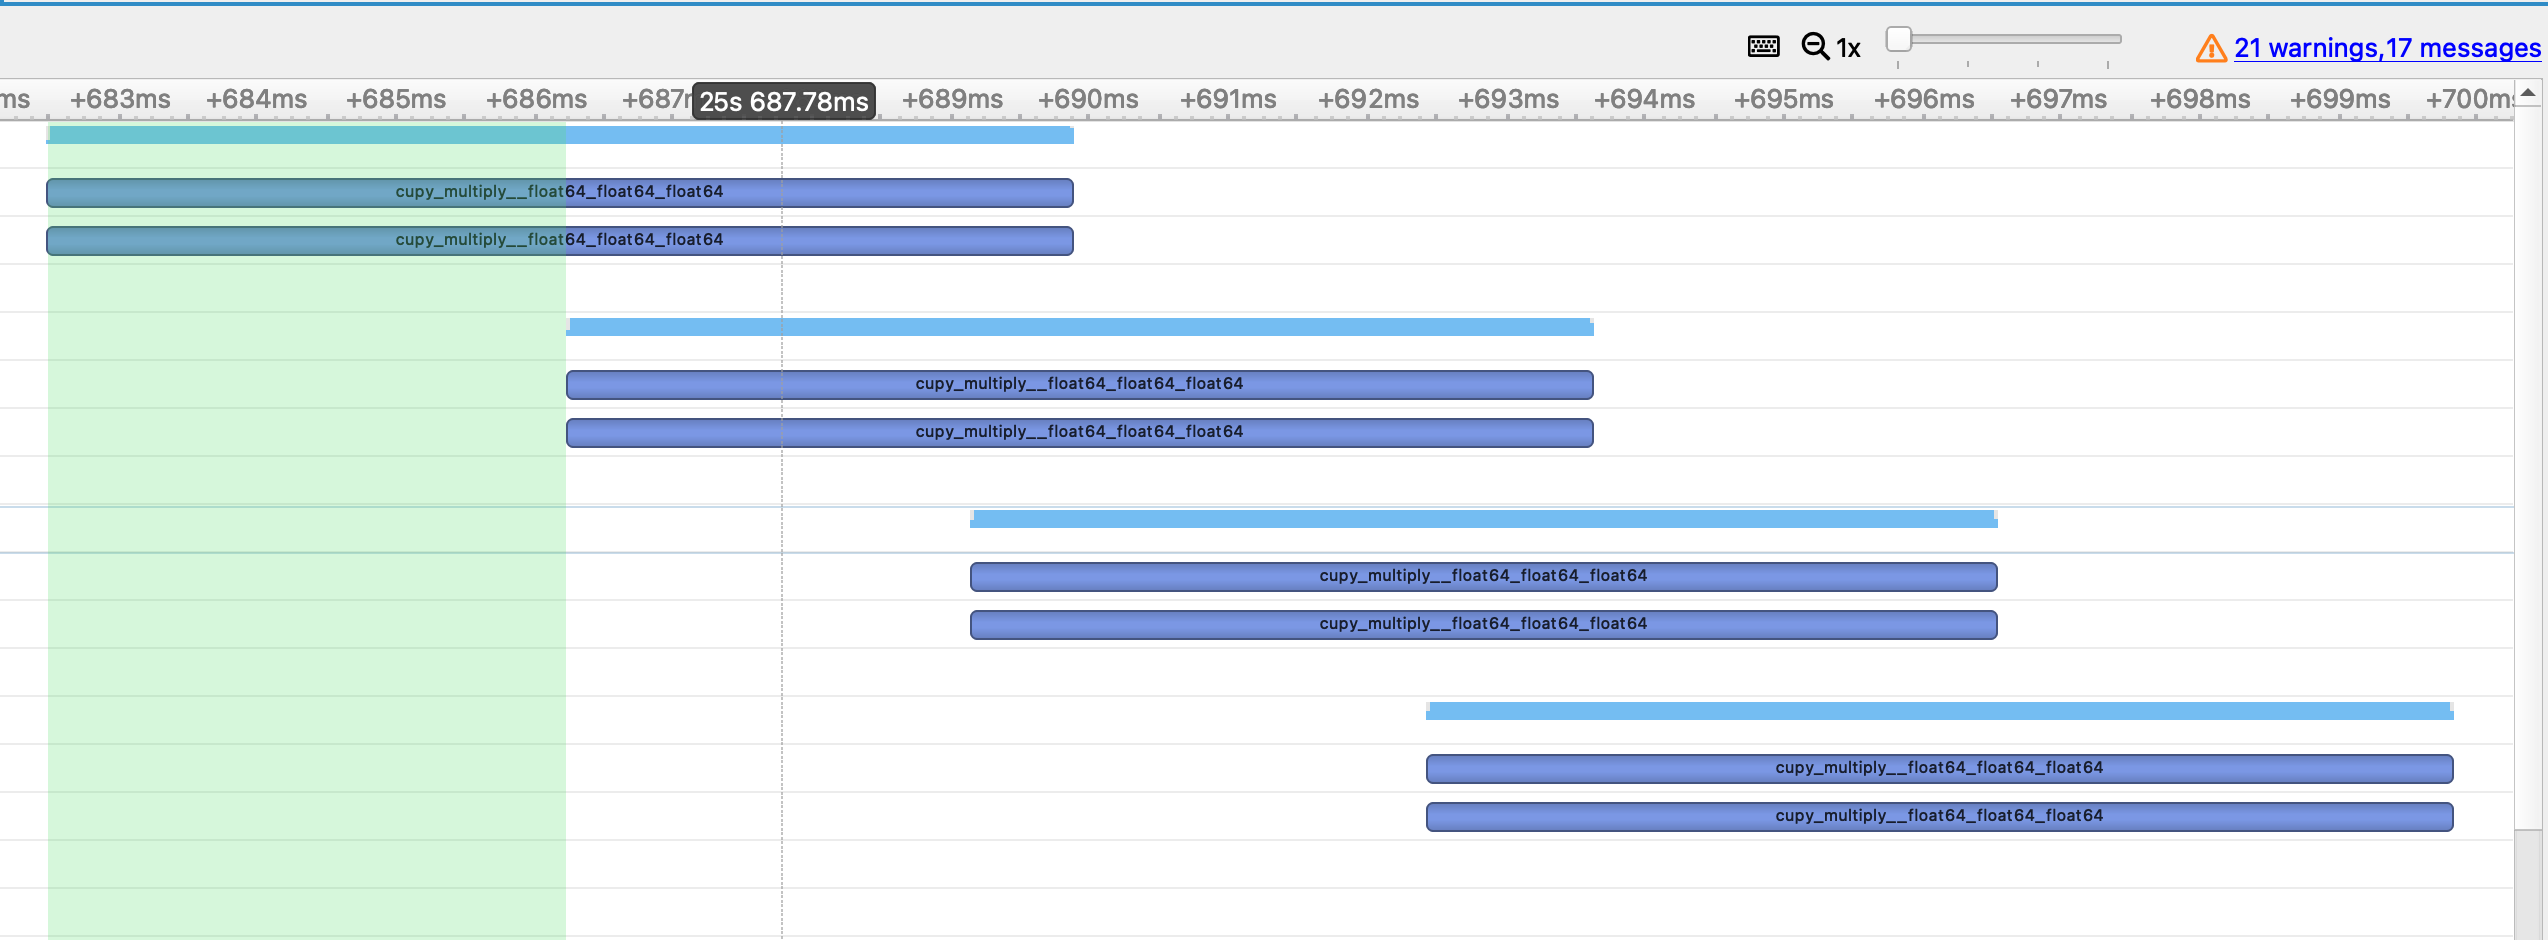
\includegraphics[width=6in]{figures/stream.png}}
  \caption{Streams not being scheduled concurrently}
\end{figure}

\subsection{Benchmarks}
For a single GPU, William analyze the Roofline model of V100 architecture theoretically and empirically. The theoretical peak observed fo NVIDIA V100 is 7833.6 GFLOP/s while the emperical peak is 7068.9 GFLOP/s \cite{roofline}. We observe by using CuPy and 
 
\section{Related Work}
For executing linear algebra in a multi-GPU systems, we see that it is still novel and in it's early stages. For example, NVIDIA's cuBLAS Multi-GPU Extension is still in it's Early Access phase to limited group of developers. \cite{cublasmg} Dask also provides multi GPU support.

https://docs.rapids.ai/api/dask-cuda/nightly/index.html

\section{Conclusions}
Currently, distributed GPU computations are still a work in progress in the current state. Although we are able to achieve good scaling with non communication algorithms, we find the performance on communication algorithms a challenge, such as matrix multiply. The limitation is not as easy to pinpoint as it could come from NVIDIA's NCCL library performance or the design of NumS. But it also ques in the work of other peopl



the main challenge in impelmenting this backend so far has been trying to optimize communication bandwidths using nvlink connenctions and non blocking communicaiton. 
https://docs.rapids.ai/api/dask-cuda/nightly/index.html

Enabling GPU support also enables users to run platform agnostic code. If users find they need faster computation or have the resourses, they can accelerate their code by just changing the backend to CPU. This can really benefit computational scientists that need to learn a new computing platform due to what their hpc provider supplies. 

\bibliographystyle{ieeetr}
\bibliography{references} 

\end{document}
